% This is samplepaper.tex, a sample chapter demonstrating the
% LLNCS macro package for Springer Computer Science proceedings;
% Version 2.20 of 2017/10/04
%
\documentclass[runningheads]{llncs}
%
\usepackage{graphicx}
% Used for displaying a sample figure. If possible, figure files should
% be included in EPS format.
%
% If you use the hyperref package, please uncomment the following line
% to display URLs in blue roman font according to Springer's eBook style:
% \renewcommand\UrlFont{\color{blue}\rmfamily}

\begin{document}
%
\title{Corridor Coupling Between Intersection Management Zones for Site-Wide Motion Co-ordination for a Fleet of Autonomous Vehicles  
\thanks{Supported by the Engineering and Physical Sciences Research Council  through a full time Doctoral Training Partnership Studentship - Institute for Transport Studies and in a Combined Award in Science and Engineering partnership with Guidance Automation Limited. 
EPSRC Project Reference 2383174. }}
%
%\titlerunning{Abbreviated paper title}
% If the paper title is too long for the running head, you can set
% an abbreviated paper title here
%
\author{Edward Derek Lambert\inst{1}\orcidID{0000-0002-2297-0441} \and
David Watling  \inst{1}\orcidID{0000-0002-6193-9121} \and
Richard Romano\inst{1}\orcidID{0000-0002-2132-4077}}
%
\authorrunning{ED. Lambert et al }
% First names are abbreviated in the running head.
% If there are more than two authors, 'et al.' is used.
%
\institute{Institute for Transport Studies, University of Leeds, 34-41 University Road, Leeds, West Yorkshire LS2 9JT UK
\email{\{tsedl, D.P.Watling, R.Romano\}@leeds.ac.uk}
\url{https://environment.leeds.ac.uk/transport} }
%
\maketitle              % typeset the header of the contribution
%
\begin{abstract}
The abstract should briefly summarize the contents of the paper in
150--250 words.

\keywords{Modelling \and  Analysis \and Safety Validation \and Robot Communication \and Autonomous Vehicles \and Collective Field Robotics}
\end{abstract}
%
%
%
%\subsection{A Subsection Sample}
%Please note that the first paragraph of a section or subsection is
%not indented. The first paragraph that follows a table, figure,
%equation etc. does not need an indent, either.
%
%Subsequent paragraphs, however, are indented.
%
\section{Introduction}
%Vehicle routing is distinguished from scheduling according to \cite{Beck2003}.
Collaborative mobile robots are being adopted widely in distribution centres and factories to increase efficiency and reduce operating costs \cite{Azadeh2019}. Models indicate they are most beneficial to e-commerce pick-pack-and-ship warehouses where the existing pick density is low \cite{Meller2018}. In this situation, adding a number of automated trolleys to ferry items back to the packing station can reduce the time pickers spend walking backwards and forwards, freeing them up to pick more items.

\begin{figure}[htbp]
\centerline{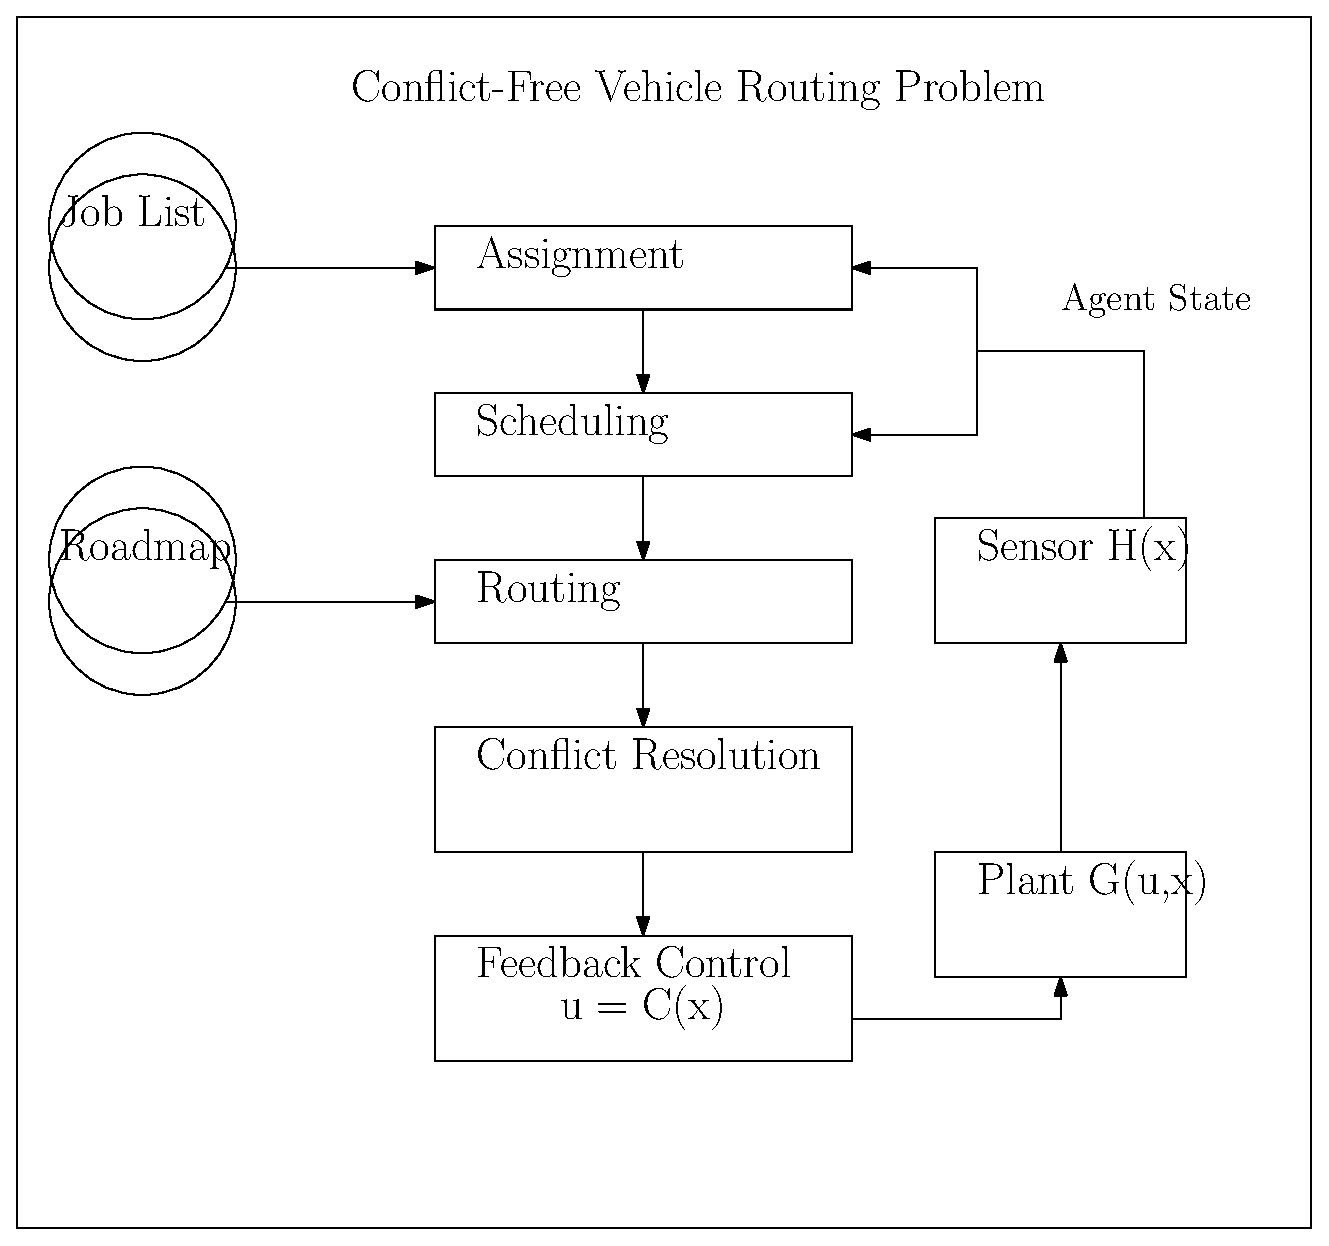
\includegraphics[width=0.7\linewidth]{dcfvrp_logical_blocks.eps}}
\caption{Possible logical division of Fleet Control tasks}
\label{fig:logical_blocks}
\end{figure}
A roadmap-based mobile robot system is a frequently used in material handling, although recently more advanced vehicles are able to take on more of the decision making, and in some cases plan their motion without supervision making them Autonomous Mobile Robots (AMR) \cite{Fragapane2021}. The fleet operator is likely to desire the most items transported in a set time, given a fixed amount of floor space. This leads to a key objective of maximum throughput for the whole site or equivalently minimum makespan \cite{Lamballais2017}.    

A fully decentralized and complete solution for controlling a fleet of autonomous mobile robots, not restricted to guide paths is given by Draganjac et al \cite{Draganjac2020}. Planning is divided into a topological layer and a more detailed private zone, a dense lattice of smooth radial polynomial paths. Live-locks are avoided as topological plans are fixed so AMR continue along the shortest topological path. Conflicts are handled and the lower layer with prioritized local negotiations in private zones. The two layers address the Routing and Conflict Resolution components of the overall fleet control problem shown in Figure \ref{fig:logical_blocks}. Deadlocks are ruled out as each local zone contains an avoidance state reachable within one move. There is also an explicit circular-wait detection procedure within the published algorithm. Results for 50 vehicles in simulation demonstrate the scalability of this approach, where a centralized algorithm might require many seconds to compute a set of safe trajectories for 10 vehicles. 

One drawback of decentralized methods comes from the time spent negotiating at each intersection. Experiments show an average negotiation time of several seconds, and a number of conflicts increase with the number of vehicles \cite{Draganjac2020}. Reducing the number of negotiations is the motivation for the intersection control based solution described by Digani et al \cite{Digani2019}. The test environment used fixed guide paths, but modern AMR resemble autonomous vehicles which may one day operate on public roads, for which Autonomous Intersection Management has been well studied. 

Car-following conflicts are resolved by the centralized routing algorithm in the reference `Full-Control' Fleet Adapter available within the Open Source Robotic Foundation's Robotic Middleware Framework (RMF) as of May 2021 cite{Vijay2021}. This is consistent with wider industry practice for roadmap-based systems reported in \cite{Fragapane2021}. Another notable adapter is the MiR 100 Fleet adapter, which 

With roadmap-reservation based collision avoidance, the following vehicle must wait until the leader has completely vacated a private zone before the follower may progress. This behaviour is convenient because it extends safely to crossing traffic without modification. The concept is simple and offers flexibility as the size of the private zone can be tuned to achieve closer spacing where desired, for example in \cite{Walenta2017} there are two zone sizes depending on whether the direction of travel is the same or not. This is a good approximation to car-following, and notable for its decentralized design too. A follow up study to investigate the added messaging overhead and potential for negotiation delay, notwithstanding, this solution could offer throughput advantages.

Research in to AIM for near future Autonomous Vehicles offers an alternative vision for collision avoidance, seemingly suitable to the most recent AMR, with a high level of autonomy. A recent review is given by Zhong et al \cite{Zhong2020}. In the AIM literature it is unusual to consider car-following conflicts, perhaps because autonomous vehicles suitable for operation on public roads are assumed to execute this function using their own sensors, perhaps in a similar way to the Adaptive Cruise Control assistance feature available in many production vehicles. Even so, the impact of interactions between vehicles are likely to be important to ensure the safe operation across the intersection. For example, even smart AMR who can overtake a lead vehicle if the AIM requests a different arrival order may well take longer to arrive, traverse a different path, or even be completely prevented from doing so by opposing traffic or vary narrow aisles. 

Zhong et al \cite{Zhong2020} includes a summary table of AIM approaches, which indicates that little attention has been given to the corridor coordination layer.  One of the few works addressing interactions between intersection zones is \cite{Du2018} which uses a 3-layer hierarchy where the manager of each intersection sends the average traffic density to its neighbours, chooses speeds within its zone of influence to minimize deviation from average road velocity, subject to the constraint that conflicts are avoided in the single zone spanning the intersection. 

With the AIM messages interface from \cite{Levin2017} the car-following constraints are a potential mechanism for implementing ``corridor coordination'' . Other works have investigated the car-following behaviour \cite{Bichiou2019} using the RPA model, which accounts for vehicle dynamic limitations. 



Using AIM to guarantee intersection safety, there is an opportunity to improve throughput by following more closely. 
 
The remaining research questions of interest to improve decentralized control of mobile robot fleets are:\\
1.  What are the performance implications of a conflict avoidance scheme based on platooning and AIM? \\
2. What are the implication for Stability/Correctness corridor coordination is used to extend this across a whole site?
3.  Which is preferable in high traffic situations?\\










\section{Method}
\section{Simulation Results}
\section{Concluding Remarks and Further Work}  
%\subsubsection{Sample Heading (Third Level)} Only two levels of
%headings should be numbered. Lower level headings remain unnumbered;
%they are formatted as run-in headings.
%
%\paragraph{Sample Heading (Fourth Level)}
%The contribution should contain no more than four levels of
%headings. Table~\ref{tab1} gives a summary of all heading levels.
%
%\begin{table}
%\caption{Table captions should be placed above the
%tables.}\label{tab1}
%\begin{tabular}{|l|l|l|}
%\hline
%Heading level &  Example & Font size and style\\
%\hline
%Title (centered) &  {\Large\bfseries Lecture Notes} & 14 point, bold\\
%1st-level heading &  {\large\bfseries 1 Introduction} & 12 point, bold\\
%2nd-level heading & {\bfseries 2.1 Printing Area} & 10 point, bold\\
%3rd-level heading & {\bfseries Run-in Heading in Bold.} Text follows & 10 point, bold\\
%4th-level heading & {\itshape Lowest Level Heading.} Text follows & 10 point, italic\\
%\hline
%\end{tabular}
%\end{table}
%
%
%\noindent Displayed equations are centered and set on a separate
%line.
%\begin{equation}
%x + y = z
%\end{equation}
%Please try to avoid rasterized images for line-art diagrams and
%schemas. Whenever possible, use vector graphics instead (see
%Fig.~\ref{fig1}).
%
%\begin{figure}
%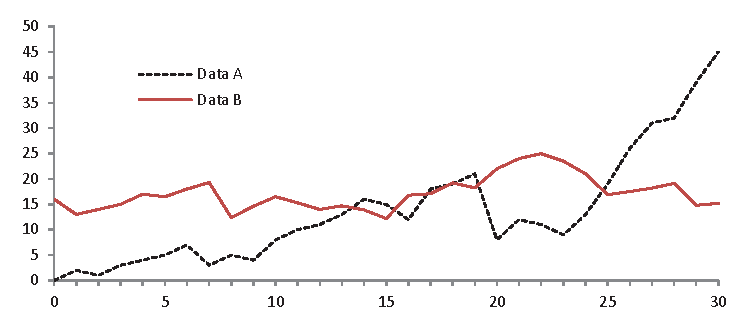
\includegraphics[width=\textwidth]{fig1.eps}
%\caption{A figure caption is always placed below the illustration.
%Please note that short captions are centered, while long ones are
%justified by the macro package automatically.} \label{fig1}
%\end{figure}
%
%\begin{theorem}
%This is a sample theorem. The run-in heading is set in bold, while
%the following text appears in italics. Definitions, lemmas,
%propositions, and corollaries are styled the same way.
%\end{theorem}
%%
%% the environments 'definition', 'lemma', 'proposition', 'corollary',
%% 'remark', and 'example' are defined in the LLNCS documentclass as well.
%%
%\begin{proof}
%Proofs, examples, and remarks have the initial word in italics,
%while the following text appears in normal font.
%\end{proof}
%For citations of references, we prefer the use of square brackets
%and consecutive numbers. Citations using labels or the author/year
%convention are also acceptable. The following bibliography provides
%a sample reference list with entries for journal
%articles~\cite{ref_article1}, an LNCS chapter~\cite{ref_lncs1}, a
%book~\cite{ref_book1}, proceedings without editors~\cite{ref_proc1},
%and a homepage~\cite{ref_url1}. Multiple citations are grouped
%\cite{ref_article1,ref_lncs1,ref_book1},
%\cite{ref_article1,ref_book1,ref_proc1,ref_url1}.
%
% ---- Bibliography ----
%
% BibTeX users should specify bibliography style 'splncs04'.
% References will then be sorted and formatted in the correct style.
%
\bibliographystyle{splncs04}
\bibliography{taros_references}

\end{document}
